\documentclass[conference]{IEEEtran}
\IEEEoverridecommandlockouts
% The preceding line is only needed to identify funding in the first footnote. If that is unneeded, please comment it out.
\usepackage{cite}
\usepackage{amsmath,amssymb,amsfonts}
\usepackage{algorithmic}
\usepackage{graphicx}
\usepackage{textcomp}
\usepackage{xcolor}
\def\BibTeX{{\rm B\kern-.05em{\sc i\kern-.025em b}\kern-.08em
    T\kern-.1667em\lower.7ex\hbox{E}\kern-.125emX}}
\begin{document}

\title{Taller-3-4 Buscador
{\footnotesize \textsuperscript{}}
\thanks{}
}

\author{\IEEEauthorblockN{1\textsuperscript{st} Juan Esteban Pinzon Preciado }
\IEEEauthorblockA{\textit{} 
\textit{Fundación Universitaria Konrad Lorenz}\\
Bogotá, Colombia \\
Juane.Pinzonp@konradlorenz.edu.co}
}
\maketitle

\begin{abstract}
Esta publicación proporcionará detalles sobre el desarrollo y la implementación de ambos algoritmos. Además, se explorará el papel de los índices invertidos en la recuperación de información, destacando su papel fundamental en los motores de búsqueda y el procesamiento de textos a gran escala. Utilizando estos algoritmos y su comprensión de los índices invertidos, se pretende mejorar la capacidad para analizar y extraer información valiosa de grandes cantidades de datos de texto.
\end{abstract}
\begin{IEEEkeywords}
Optimización, recursos, lógica, complejidad, análisis
\end{IEEEkeywords}

\section{Introducción}
La capacidad de procesar y analizar eficazmente grandes conjuntos de datos de texto desempeña un papel crítico en campos como el procesamiento del lenguaje natural y la recuperación de información. En este artículo, exploraremos algoritmos diseñados para abordar dos tareas fundamentales en este contexto: la clasificación de palabras más frecuentes y la recuperación de documentos que contienen palabras clave específicas. Estos algoritmos utilizan conceptos como la memorización y la indexación inversa para mejorar la capacidad de extraer información valiosa de vastos volúmenes de datos de texto.

A lo largo de este análisis, examinaremos en detalle el código y sus componentes para comprender cómo estos algoritmos pueden ser implementados de manera efectiva. Además, exploraremos su utilidad en aplicaciones prácticas, como motores de búsqueda y análisis de texto a gran escala. Al final de este artículo, habremos adquirido una comprensión sólida de cómo estos algoritmos pueden contribuir significativamente a la mejora del procesamiento de datos textuales.

\section{Análisis código }

\subsection{Ocurrencia de palabras}
\begin{verbatim}
def contar_ocurrencias(palabra, diccionario):
    if palabra not in diccionario:
        return 0
    ocurrencias = 0
    for documento in diccionario[palabra]:
        ocurrencias += documento.count(palabra)
    return ocurrencias
\end{verbatim}
\vspace{3cm}
\subsection{Clasificación palabras}
\begin{verbatim}
def clasificar_palabras(diccionario):
    palabras_ordenadas = sorted(diccionario.keys(), 
        key=lambda palabra: contar_ocurrencias(palabra, diccionario), reverse=True)
    print("Clasificación de palabras más repetidas:")
    for palabra in palabras_ordenadas:
        ocurrencias = contar_ocurrencias(palabra, diccionario)
        print(f"'{palabra}': {ocurrencias} veces")
\end{verbatim}
\vspace{0.4cm}
\subsection{Ranking palabras más concurridas}
\begin{verbatim}
for documento in my_documents:
        for palabra in documento.split():
            if palabra not in diccionario:
                diccionario[palabra] = []
            diccionario[palabra].append(documento)
    clasificar_palabras(diccionario)
\end{verbatim}
\vspace{0.5cm}
\subsection{Buscar palabra en específico}
\begin{verbatim}
def buscar(diccionario, palabra_a_buscar):
    if palabra_a_buscar in diccionario:
        return diccionario[palabra_a_buscar]
    else:
        return []
\end{verbatim}
\vspace{0.4cm}
\subsection{Cargar diccionario con la información a iterar}
\begin{verbatim}
for i, documento in enumerate(my_documents):
        palabras = documento.split()
        for palabra in palabras:
            if palabra not in diccionario:
                diccionario[palabra] = [i]
            else:
                diccionario[palabra].append(i)
\end{verbatim}

\subsection{Palabra específica a buscar}
\begin{verbatim}
palabra_a_buscar = "Python"
documentos= buscar(diccionario,palabra_a_buscar)
if documentos:
    print(f"Documentos que contienen '{palabra_a_buscar}':")
    for documento_index in documentos:
        print(my_documents[documento_index])
else:
    print(f"'{palabra_a_buscar}' no se encontró")
    
\end{verbatim}

\section{Código}

\begin{figure}[h]
  \centering
  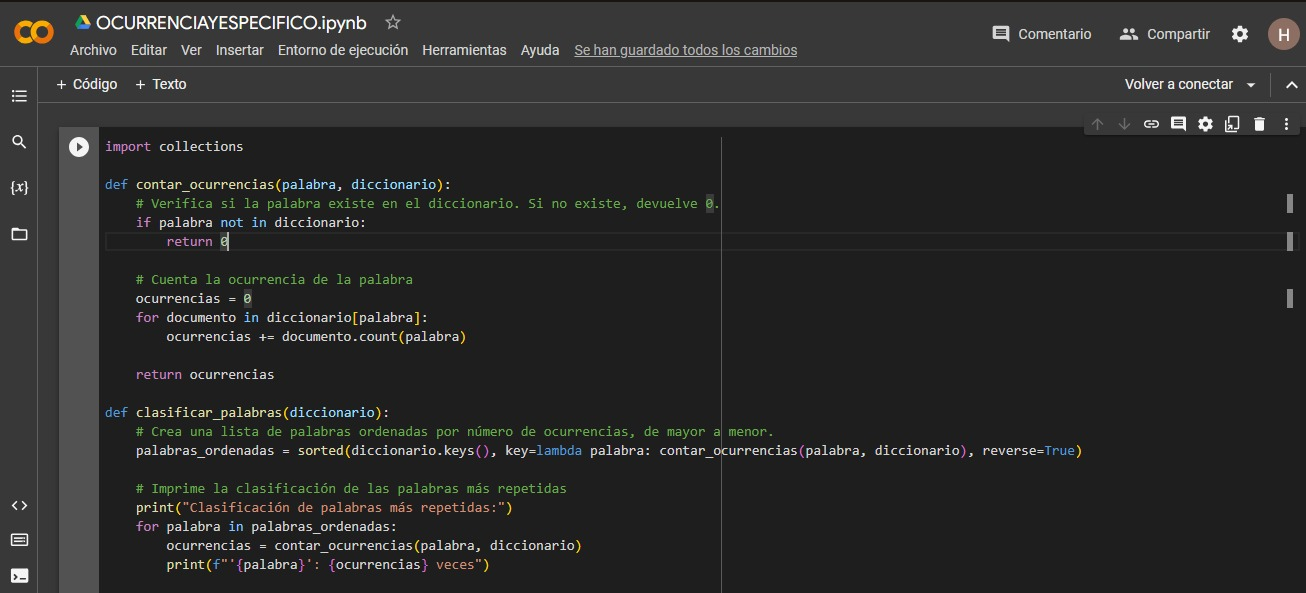
\includegraphics[width=9cm]{WhatsApp Image 2023-09-11 at 9.14.40 PM.jpeg}
  \caption{Importaciones y creación de biblioteca para los datos.}
  \label{fig:importaciones}
\end{figure}

\begin{figure}[h]
  \centering
  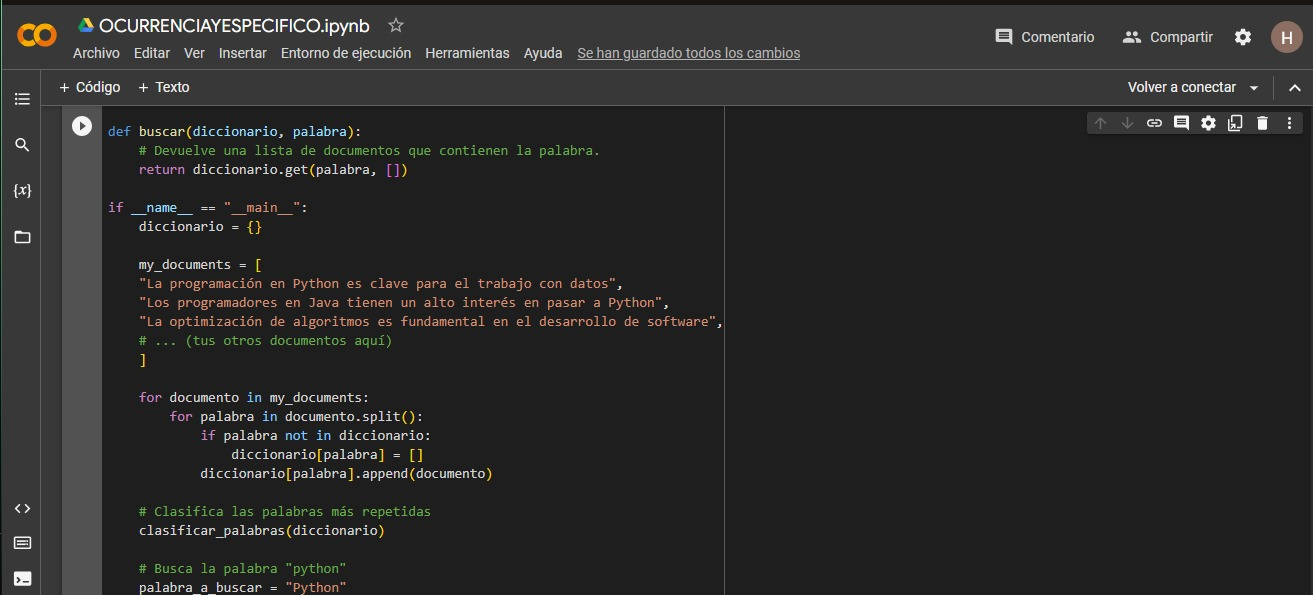
\includegraphics[width=9cm]{WhatsApp Image 2023-09-11 at 9.14.58 PM.jpeg}
  \caption{Se realiza el ciclo para que pase por cada una de las palabras.}
  \label{fig:ciclo}
\end{figure}

\begin{figure}[h]
  \centering
  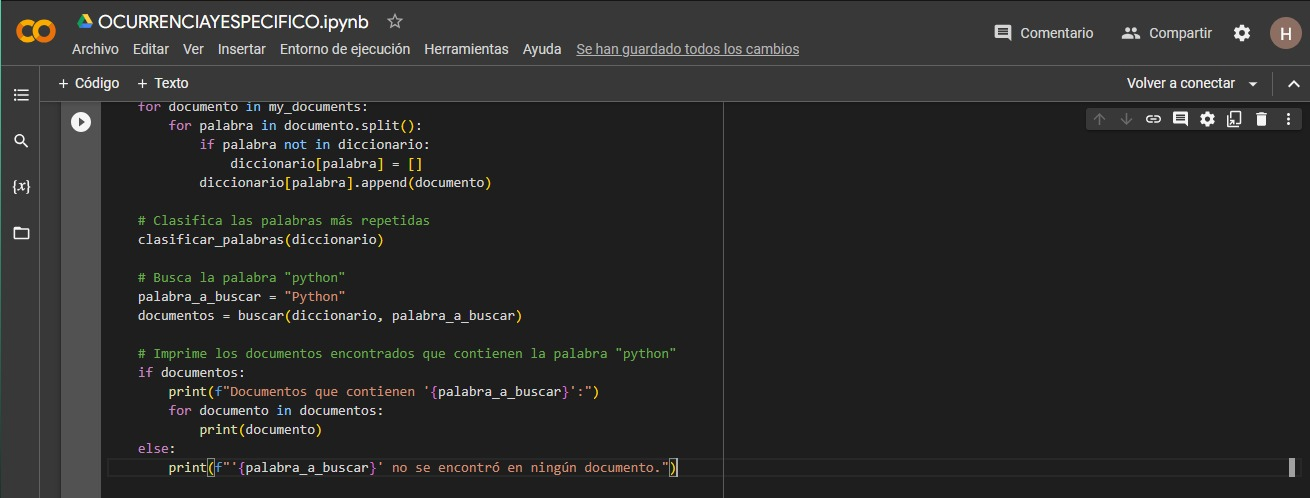
\includegraphics[width=9cm]{WhatsApp Image 2023-09-11 at 9.15.10 PM.jpeg}
  \caption{Clasificación de palabras.}
  \label{fig:clasificacion}
\end{figure}
\vspace{5cm}

\begin{figure}[h]
  \centering
  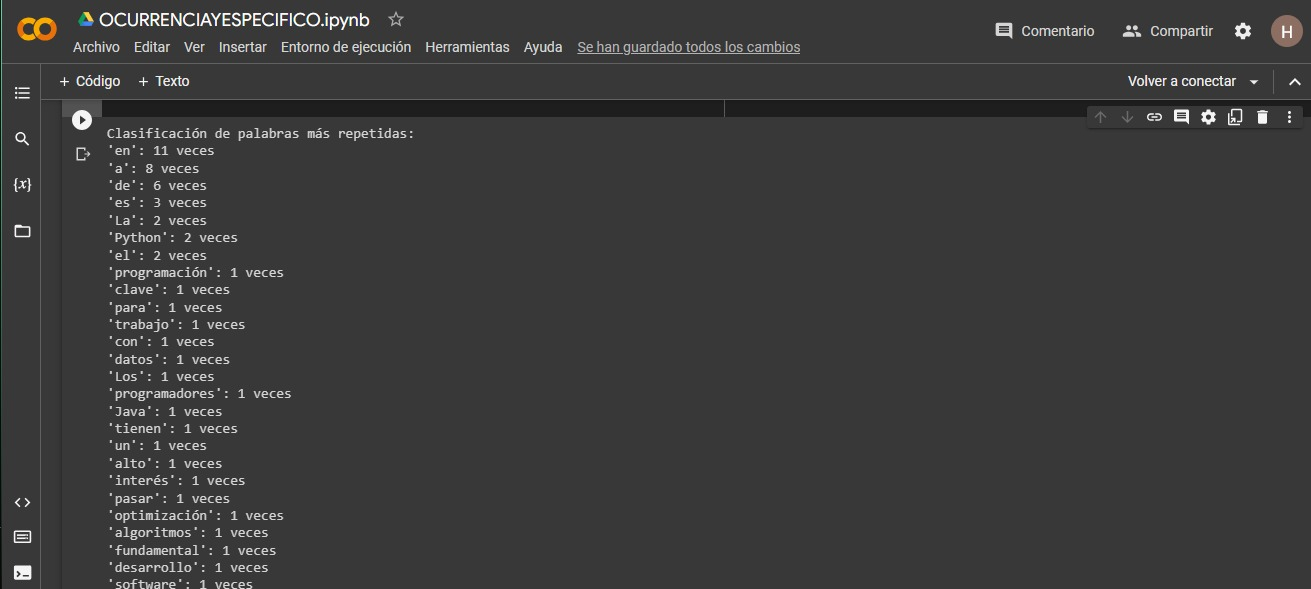
\includegraphics[width=9cm]{WhatsApp Image 2023-09-11 at 9.15.23 PM.jpeg}
  \caption{Palabras más repetidas.}
  \label{fig:repetidas}
\end{figure}

\begin{figure}[h]
  \centering
  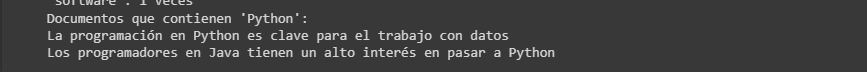
\includegraphics[width=9cm]{WhatsApp Image 2023-09-11 at 9.15.41 PM.jpeg}
  \caption{Búsqueda de la palabra.}
  \label{fig:busqueda}
\end{figure}

\section{Conclusiones}
\begin{enumerate}
  \item \textbf Este código proporciona una funcionalidad eficiente y versátil para el procesamiento de grandes volúmenes de datos de texto. Su implementación sencilla lo hace adecuado para una variedad de aplicaciones, desde la clasificación de palabras hasta la recuperación de documentos. Su capacidad para manejar grandes conjuntos de datos lo convierte en una herramienta valiosa en un entorno de información en constante crecimiento. La utilización de diccionarios permite una relación efectiva entre palabras y los documentos que las contienen, garantizando un acceso rápido y eficiente a la información relevante. Además, la presentación ordenada de las palabras más frecuentes junto con sus apariciones contribuye a una comprensión clara de los datos, lo que resulta especialmente valioso en aplicaciones relacionadas con la búsqueda y el análisis de texto. En resumen, este código es una solución eficiente y versátil que puede ser una base sólida para proyectos de investigación y desarrollo en el campo del procesamiento de lenguaje natural y la recuperación de información.






\end{enumerate}

\end{document}
